\index{Validate Model}
\index{Modeling!Validate}

You can validate your model at any time by selecting:\\
\bxmenu{Modeling}{Validate}{}. \\


Or by clicking the \bxcaption{validate} button on the toolbar.
The validation ensures that the model is fit to be generated, and does not contain any errors. 
\gdmarpar{../../../share/PS/validate}{Validate}

If there are errors in the model, you will see this in the console output. In the \gdmodeleditor{} itself, the places with errors will be marked with a red cross. Hovering over the cross will show a tooltip with information on the error (\bxfigref{ModelError}). 

\begin{figure}
\begin{center}
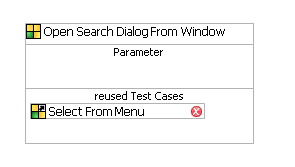
\includegraphics{Tasks/Modelling/PS/ModelError}
\caption{Model showing an error}
\label{ModelError}
\end{center}
\end{figure} 
